\section{Network Configuration} \label{sec:Network Configuration}

Within this section we introduce our system. We define a temporal liquid state
machine (TLSM) as an input vector, encoded in time-based spikes, followed by a
reservoir of temporal neurons, and finally a singular output column (with
winner-takes-all lateral inhibition). The input vector uses encoding strategies
discussed in \cite{Encoding}, and the output column is identical to the one
described in \cite{TNN}.

\begin{figure}[h]
    \centering
    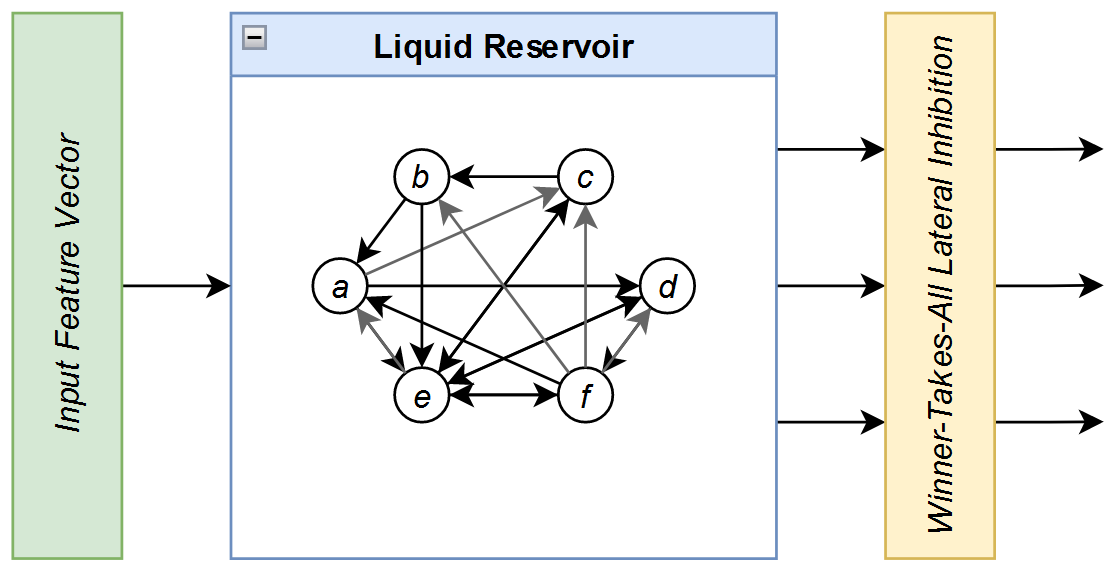
\includegraphics[scale=0.25]{tlsm_diagram.png}
    \caption{Diagram of a temporal liquid state machine (TLSM).}
    \label{fig:tlsm_diagram}
\end{figure}

\subsection{Input Encoding}

The input vector is a series of time-encoded one-hot vector spikes. For MNIST
data, the input $28 \times 28$ image is flattened into a $784 \times 1$ vector.
Each element of the vector is subsequently expanded into a $t_{res} \times 1$
one-hot time-spike encoding vector, where the time represents a pixel's
brightness. If the pixel is simply black, the time is set to zero; Any low
values will also round to zero. Higher values may round to higher indices.

More and different input processing techniques may be necessary in order to
improve the accuracy of the network, which is not a focus of this project. For
instance, in order to ensure that bright pixels do not 'dominate' the input, the
image may be duplicated and inverted to include a pos-neg encoding scheme,
resulting in a $1568 \times 1$ input vector. Furthermore, completely zeroed
input values may be removed from the input vector, encoding the input time as
$t = \infty$. As the focus of the project is the network arrangement and not the
network's accuracy at classifying digits, we leave these techniques to future
consideration.

The temporal resolution, $t_{res}$, is an important hyperparameter of this
encoding scheme, as with higher resolutions the network may take longer to train
and infer. However, as resolution increases, so too does accuracy. We set this
value to $t_{res} = 10$ for our implementation.

\subsection{Temporal Neuron} \label{sec:Temporal Neuron}

The temporal neuron is a simple model of a neuron that fires in response to a
series of time-spiking encoded inputs. It is mainly discussed in \cite{TNN}, but
we will briefly summarize its functionality here. Chiefly, the temporal neuron
consumes significantly less power than point-integrator alternatives, and is
generally trained in an unsupervised fashion. The temporal neuron is also
considered a more biologically plausible neuron model, as it more closely
relates to the Hodgkin-Huxley model \cite{Hodgkin-Huxley} of a neuron.

The temporal neuron takes in a series of inputs on a number of lines, generally
encoded in a one-hot manner. Each line has an internal weight represented with
it, encoding the dendritic segment's channel strength from the pre-synaptic
neuron. The input lines are multiplied and summed, and the result increases the
neuron's body potential. When the body potential reaches a threshold $\theta$,
the neuron will spike, sending a high signal on its axonal output line, and the
body potential will reset.

The method in which neurons accumulate body potential is a potential
hyperparameter of temporal network design. We implement the Step No-Leak (SNL)
neuron in this work, which simply instantly increases the body potential based
on the incoming potentials from the dendritic segments (inputs). A more involved
strategy is the Ramp No-Leak (RNL) neuron model, where body potential will
increase over time corresponding to the input and weight. The Leaky
Integrate-and-Fire (LIF) neuron model is an even more biologically plausible
model, where the body potential will (in addition to the ramping nature of the
RNL neuron) 'leak' out over time, decreasing the excitation rate.

\subsection{STDP Training}

We implement Spike-Timing-Dependent Plasticity (STDP) training rules for the
temporal neurons within our work. STDP rules are based closely on Hebbian theory
\cite{STDP}, though the actual definitions of the rules vary. For our
implementation, we utilize unsupervised STDP rules as well as supervised STDP
rules as proposed in \cite{TNN} for some input spike time $t_i$ and output time
$t_j$:

$$
    \Delta w_{ij} = \begin{cases}
        \begin{matrix}
            B(\mu_c)  & \text{ if } t_i\leq t_j, &                 & t_j\neq\infty \\
            -B(\mu_b) & \text{ if } t_i > t_j,   &                 &               \\
            B(\mu_s)  & \text{ if }              & t_i\neq \infty, & t_j=\infty
        \end{matrix}
    \end{cases}
$$

The parameters of $\mu_c$, $\mu_b$, and $\mu_s$ are the STDP capture, backoff,
and search parameters. They represent finite probabilities, and the notation of
$B(\mu_*)$ refers to the choosing of a Bernoulli random variable. This
implementation of STDP is unsupervised; \cite{TNN} also proposes a supervised
approach to training called R-STDP, which will be used for an output layer.
Generally, $\mu_*$ is set to inverse powers of two. For our implementation, we
utilize $\mu_c = 2^{-3}$, $\mu_b = 2^{-7}$, and $\mu_s = 2^{-10}$. Generally,
high capture values $\mu_c$ correspond to a network's willingness to learn new
information; Lower backoff values $\mu_b$ teach the network to forget poorly
formed connections less, and lower search values $\mu_s$ are added in order to
force the network from a state of dormancy to excitation.

Alongside these, the parameters of $W_{max}$ and $W_{min}$ are the maximal and
minimal allowed weight values. After STDP training, all weights are clamped to
this particular range. These parameters are usually $W_{min} = 0$ and
$W_{max} = 2^3$. The value of $W_{max}$ corresponds to the maximal weight
resolution, and from \cite{TNN} $2^3$ is generally 'biologically enough.' From
our testing, we find insignificant benefits increasing past $2^3$, but we leave
our neurons at $2^6$ in order to slow down excitation and observe effects more
granularly.

Finally, the threshold value $\theta$ is generally defined as a function of the
number of input neurons $n_i$ and the maximal weight $W_{max}$:

$$
    \theta = \max(1, W_{max} \times n_i \times \theta_f)
$$

The value of $\theta_f$ is a hyperparameter of the network, and is bounded
within $0 < \theta_f < 1$. We set the value of $\theta_f = 0.1$, though other
higher values could slow down excitation further.

\subsection{Reservoir}

The reservoir is the focus of network analysis, containing a series of temporal
neurons arranged in a randomly connected graph, or a 'liquid'. This graph of
neurons will change over time with training and with STDP rules, adding and
removing connections arbitrarily in response to the inputs. We start with the
parameter of $n$ neurons, which we set to $n=150$ for our implementation, based
on the number of neurons loosely suggested to exist in a cortical column
\cite{Mountcastle}.

Furthermore, a 'seed' configuration for the network may be specified, indicating
its initial connectivity. This seed configuration $W_0$ is generated through a
number of random graph algorithms, and is a hyperparameter of the network. We
test on seed networks of fully connected (FC) nodes, Erdos-Renyi (ER) graphs,
Barabasi-Albert (BA) graphs, and Watts-Strogatz (WS) graphs. Each of these
networks contains their own particular parameters:

\begin{enumerate}
    \item FC: No parameters.
    \item ER: The probability of edge creation $p$.
    \item BA: The number of edges to attach from a new node $m$.
    \item WS: The probability of rewiring each edge $p$, and the number of
          edges within the base lattice $k$.
\end{enumerate}

The liquid reservoir is simulated on a time quanta for each particular and
unique training sample. On each iteration, the reservoir is fed a new spiking
column of the input vector (if it exists), and any excitations are then fed back
to the reservoir's neighboring connections. When the input vector is exhausted,
the reservoir continues until $t_{max}$, the maximal amount of time for the
quanta. The reservoir is then trained with STDP rules, before being readied for
the next quanta. The maximal amount of time in a quanta is a hyperparameter of
the network, and allows the network to 'settle' into a more favorable position
after a series of excitations. We set this value $t_{max} = 20$.

\subsection{Discriminant Column}

The output discriminating column, responsible for classifying the state of the
liquid, is implemented as a TNN minicolumn as described in \cite{TNN}. The
minicolumn is a series of $n$ neurons (for $n$ output classifications), and is
furthermore fed into a winner-takes-all lateral inhibition (WTA-LI) layer. The
WTA-LI layer implements the biological function of astroglia, inhibiting outputs
of neurons as necessary. STDP rules for this output column take into account the
output time $t_j$ as the time when the entire column spikes.

With the WTA-LI column, the first neuron to spike inhibits all other neurons,
and will dominate the output. Other forms of inhibition and astrocyte modelling
have been explored in related work (see \cite{Astrocyte}), but will not be
explored within our project.

The temporal minicolumn utilizes R-STDP rules for learning, which simply
modulate the prior cases of STDP (capture, backoff, and search) based on whether
the output matches some target value:

\begin{enumerate}
    \item If the output is correct, then STDP search is disabled; The other
          STDP rules are performed as normal.
    \item If the output is incorrect, then STDP backoff is disabled. The capture
          weights are decremented instead of incremented, and search is still enabled.
    \item If the column never spikes, only search operates.
\end{enumerate}

All other parameters for neurons ($\theta$, $W_{max}$, $W_{min}$, $\mu_*$) are
configured to be identical to the liquid's neurons for our implementation.